\documentclass[11pt,a4paper]{article}

\usepackage{../../templates/style}

\begin{document}

\begin{problem}{Runnner}{standard input}{standard output}{1 second}{16 megabytes}

นักวิ่ง $N$ คน วิ่งแข่งกันในสนามที่มีลู่วิ่ง $M$ ลู่ ก่อนการแข่งขันจะเริ่มต้น นักวิ่งจะทยอยไปยืนรออยู่ที่ลู่วิ่งโดยจะยืนรอกันตามลำดับที่เดินเข้ามาในสนาม  ในการยืนรอนี้ไม่จำเป็นที่จำนวนนักวิ่งในแต่ละลู่ต้องเท่ากัน  เมื่อนักวิ่งยืนที่ลู่ครบทุกคนแล้วการแข่งจะเริ่มขึ้น  โดยจะแบ่งเป็นรอบ ๆ ในรอบที่ $1$ นักวิ่งที่ยืนอยู่เป็นอันดับแรกของแต่ละลู่วิ่งจะวิ่งแข่งกัน คนที่มีความเร็วสูงที่สุดจะเป็นผู้ชนะ จากนั้นในรอบถัดมานักวิ่งคนถัดไปของทุกลู่วิ่งจะวิ่ง  การแข่งขันจะดำเนินไปเรื่อย  ๆจนกระทั่งนักวิ่งทุกคนออกวิ่ง

\bigskip
\underline{\textbf{โจทย์}}  ให้เขียนโปรแกรมรับข้อมูลการเดินเข้าลู่วิ่งของนักวิ่งแต่ละคน พร้อมด้วยอัตราเร็วในการวิ่ง  จากนั้นให้โปรแกรมคำนวณหาผู้ชนะในการวิ่งแต่ละรอบจนครบทุกรอบ

\InputFile

\textbf{บรรทัดแรก} ประกอบด้วยจำนวนเต็ม $N$ และ $M$  $(1 \leq N \leq 100\,000; 1 \leq M \leq 10\,000)$

\textbf{บรรทัดที่ $2$ ถึง $N+1$} จะเป็นข้อมูลการเดินเข้าสนามและความเร็วของนักวิ่งแต่ละคน กล่าวคือ ในบรรทัดที่ $i+1$  จะเป็นข้อมูลของนักวิ่งที่เดินเข้าสนามมาเป็นลำดับที่ $i$ บรรทัดดังกล่าวประกอบไปด้วยจำนวนเต็ม $A_i$ $L_i$ $S_i$  โดยที่ $A_i$ คือหมายเลขของนักแข่งซึ่งจะไม่ซ้ำกัน  $L_i$ แทนหมายเลขลู่ที่เขาเดินไปรอ และ $S_i$ แทนความเร็วของนักวิ่ง  $(1 \leq A_i \leq 1\,000\,000; 1\leq L_i \leq M; 1\leq S_i \leq 1\,000\,000)$

\OutputFile

\textbf{มีหลายบรรทัด} ผลลัพธ์จะมีจำนวนบรรทัดเท่ากับจำนวนรอบของการแข่งขัน ในแต่ละบรรทัด $j$ ให้พิมพ์หมายเลขของนักวิ่งที่ชนะในรอบที่ $j$  นักวิ่งที่ชนะในรอบที่ $j$ คือคนที่มีอัตราเร็วสูงสุดที่วิ่งในรอบนั้น  ถ้านักวิ่งที่มีอัตราเร็วมากที่สุดมีมากกว่าหนึ่งคน ให้ตอบคนที่อยู่ในลู่วิ่งที่มีหมายเลขน้อยที่สุด

\Examples

\begin{example}
\exmp{6 3
1 1 10
2 2 5
3 2 10
4 3 10
5 1 7
6 2 7}{1
3
6}%
\end{example}

\Note

\begin{figure}[h]
\centering
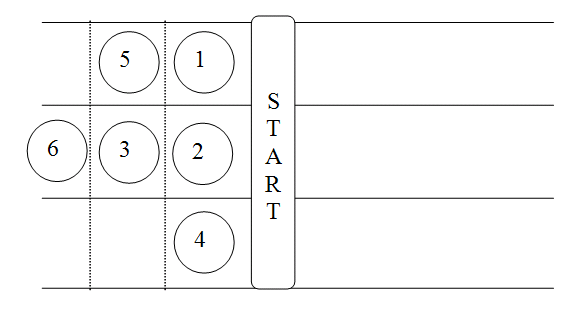
\includegraphics[width=0.7\textwidth]{../latex/img/1049/1049-1.png}
\caption{รูปประกอบตัวอย่างข้อมูลนำเข้า}
\end{figure}

\Scoring

\textbf{ใน 30\% ของข้อมูลชุดทดสอบ}: $N \leq 100; M\leq 100$

\Source

สอบปฏิบัติครั้งที่ 1 ค่ายคัดเลือกผู้แทนประเทศไทย ไปแข่งขันคอมพิวเตอร์โอลิมปิกระหว่างประเทศปี 2550 ค่ายที่ 1

\end{problem}

\end{document}